% DRAFT for arXiv (quant-ph). Not submitted.
% Before submitting: fill in the author block, read every line, confirm the acknowledgment,
% and remove the DRAFT line under the title.
\documentclass[11pt]{article}
\usepackage[margin=1in]{geometry}
\usepackage{amsmath,amssymb,amsthm}
\usepackage{graphicx}
\usepackage[colorlinks=true,linkcolor=blue,citecolor=blue,urlcolor=blue]{hyperref}

\newtheorem{theorem}{Theorem}
\newtheorem{proposition}[theorem]{Proposition}
\newtheorem{corollary}[theorem]{Corollary}
\theoremstyle{remark}
\newtheorem{remark}[theorem]{Remark}

\newcommand{\R}{\mathbb{R}}
\newcommand{\C}{\mathbb{C}}
\newcommand{\one}{\mathbb{1}}
\newcommand{\tr}{\operatorname{tr}}

\title{Only energy differences matter:\\ a single imaginary unit for quantum dynamics over the reals}
\author{Brennan Pope\\ \small [affiliation] \quad \small [email]}
\date{}

\begin{document}
\maketitle
\begin{center}\textbf{DRAFT --- not for distribution}\end{center}

\begin{abstract}
In quantum theory over a real Hilbert space, every norm-preserving, energy-conserving dynamics carries its own complex structure, so a quarter turn $J$ with $J^2=-1$ does not by itself single out complex quantum theory. We show that one physical requirement, that shifting the energy zero changes the dynamics only by a fixed common rotation, forces a single complex structure shared by every Hamiltonian: $A(H)=JH/\hbar$ with $[J,H]=0$ for all $H$. The proof takes five lines, from antisymmetry of the generator and the Planck--Einstein relation $A(H)^2=-H^2/\hbar^2$; energy conservation follows. Each input can be weakened. The energy-zero requirement follows from asking that the dynamics of two non-interacting systems depend only on their total Hamiltonian. Antisymmetry follows from stability, given that observables can serve as Hamiltonians and fix states up to phase. The Planck--Einstein relation follows from asking only that an energy eigenstate's rotation rate be a fixed function of its energy: the rate is forced to be $|E-E_0|/\hbar$, with $\hbar$ a constant, once one level is non-degenerate or the system is composed with another. Where the assumption that observables can serve as Hamiltonians is used to make them commute with $J$, it can be replaced by the requirement that a shift of the energy zero change no measured average. Consequences: real quantum theory with all symmetric observables violates the requirement, as does quaternionic quantum theory with quaternion-linear dynamics, and for two non-interacting subsystems the requirement gives $J_A\otimes 1=1\otimes J_B$, which reduces the real tensor product to the complex one. The three recent real formulations that reproduce all multipartite predictions each satisfy our assumptions and contain the shared $J$ explicitly, so the theorem explains their agreement with experiment.
\end{abstract}

\section{Introduction}

Why does quantum mechanics use complex numbers? A common intuition is that quantum time evolution is a rotation and rotations need an imaginary unit. That intuition is incomplete. Norm preservation makes the generator of time evolution antisymmetric on a real Hilbert space, and every antisymmetric operator comes with a natural complex structure on its non-degenerate part (its polar part, the ``positive-frequency'' complex structure \cite{AshtekarMagnon,Aste,Vaughan}). Real quantum theory therefore already has a $J$ for each dynamics. What it lacks is a \emph{single} $J$, common to all Hamiltonians and commuting with every observable, which is what the imaginary unit of complex quantum theory provides. Stueckelberg postulated such a universal $J$ \cite{Stueckelberg}; Moretti and Oppio derived one for relativistic elementary systems from Poincar\'e symmetry \cite{MorettiOppio}. In operational frameworks, a link between observables and generators of dynamics singles out complex quantum theory \cite{AlfsenShultz,BMU}.

The question has become sharper since Renou \emph{et al.} showed that real quantum theory with the standard real tensor product makes different predictions from complex quantum theory in a network scenario \cite{Renou}, a difference confirmed experimentally \cite{Chen,Li}. Real formulations with modified composition rules have since been proposed that reproduce all multipartite predictions \cite{HoffreumonWoods,BarriosHita,MaioliCuradoGazeau}, while others argue that such formulations carry a hidden complex structure \cite{BangChoBaek} or require nonlocal maps \cite{FengRenVedral}.

Here we give a short argument that isolates the physical requirement that makes the complex structure universal. It is the elementary fact that only energy differences are physical: shifting a Hamiltonian by a constant, $H\mapsto H+c\one$, should change the dynamics only by a common rotation, $A(H+c\one)=A(H)+cA(\one)$. Together with the Planck--Einstein relation, this forces $A(H)=JH/\hbar$ with one $J$ for every $H$ (Theorem~\ref{thm:main}). The same requirement, applied to a shift of total energy in a composite system, fixes the composition rule (Proposition~\ref{prop:composite}). Conversely, the requirement is itself forced by composition: a constant added to the total energy of two non-interacting systems is the same joint Hamiltonian whichever part it is booked to, and if the joint dynamics depends only on the joint Hamiltonian, the resulting common rotation cannot depend on either part's own Hamiltonian (Proposition~\ref{prop:shift}). Where the assumption that every observable is a possible Hamiltonian serves to make observables commute with $J$, it can be replaced by the same principle stated for measurements: shifting the energy zero changes no measured average (Remark~\ref{rem:a0}). Norm preservation can also be weakened to stability, the requirement that no state grows without bound, given that the observables determine states up to the common phase (Proposition~\ref{prop:stable}). Even the Planck--Einstein relation need not be assumed in full: if the rotation rate of an energy eigenstate is any fixed function of its energy, the energy-zero requirement forces it to be $|E-E_0|/\hbar$, with $\hbar$ a constant read off from that function, as soon as one Hamiltonian has a non-degenerate level or the system can be composed with another (Propositions~\ref{prop:pe} and~\ref{prop:nogap}); composition also makes $\hbar$ the same for every system.

\section{Setting and assumptions}

Let the state space be $\R^n$ with the standard inner product, states being unit vectors. Observables are symmetric matrices. Let $\mathcal{H}$ be the set of Hamiltonians, a set of symmetric matrices that contains $\one$ and is closed under $H\mapsto H+c\one$ for real $c$. Each $H\in\mathcal{H}$ generates linear dynamics $\dot\psi = A(H)\psi$. We assume, for all $H\in\mathcal{H}$:

\begin{itemize}
\item[(A0)] Every observable can serve as a Hamiltonian: every observable lies in $\mathcal{H}$.
\item[(A1)] \emph{Norm preservation:} $A(H)^{T}=-A(H)$.
\item[(A2)] \emph{Energy conservation:} $[A(H),H]=0$.
\item[(A3)] \emph{Planck--Einstein:} $A(H)^2=-H^2/\hbar^2$. Given (A1) and (A2), which follows (Theorem~\ref{thm:main}), this says that on each energy eigenspace of $H$, with energy $E$, the dynamics is a rotation at angular frequency $|E|/\hbar$. Proposition~\ref{prop:pe} weakens it to the requirement that the frequency be some fixed function of $E$.
\item[(A4)] \emph{Only energy differences matter:} $A(H+c\one)=A(H)+c\,A(\one)$ for every real $c$.
\end{itemize}

(A1) and (A2) are the standard requirements of reversible, energy-conserving evolution \cite{Vaughan}. We list (A2) because it is standard, but it is not an independent assumption: Theorem~\ref{thm:main} derives it from (A3) and (A4). (A4) says that a constant shift of the energy zero has no effect beyond a common rotation of all states, the same for every $H$. (A3) fixes only the magnitude of each rotation rate; (A4) is what ties the sense of rotation to the sign of the energy. Complex quantum theory, written over the reals with $i$ replaced by a real orthogonal $J$ with $J^2=-\one$, satisfies (A0)--(A4) with $A(H)=JH/\hbar$ and observables the symmetric matrices commuting with $J$.

\section{One complex structure for all Hamiltonians}

\begin{theorem}\label{thm:main}
Under (A1), (A3) and (A4), there is a single real matrix $J$ with $J^T=-J$ and $J^2=-\one$ such that, for every $H\in\mathcal{H}$,
\begin{equation}
[J,H]=0 \qquad\text{and}\qquad A(H)=\frac{1}{\hbar}JH .
\end{equation}
In particular energy conservation (A2) holds, $n$ is even, and $\hbar\dot\psi = JH\psi$, which is the Schr\"odinger equation $i\hbar\dot\psi=H\psi$ with $i\leftrightarrow -J$.
\end{theorem}

\begin{proof}
(i) Set $J:=\hbar A(\one)$. By (A3) with $H=\one$, $J^2=-\one$, and by (A1), $J^T=-J$. A real matrix with $J^2=-\one$ exists only for even $n$.

(ii) Fix $H$ and set $B:=\hbar A(H)$. By (A4), $\hbar A(H+c\one)=B+cJ$. Applying (A3) to $H+c\one$ gives $(B+cJ)^2=-(H+c\one)^2$ for all $c$. Comparing powers of $c$:
\begin{equation}\label{eq:coeffs}
B^2=-H^2,\qquad BJ+JB=-2H .
\end{equation}

(iii) Since $J^2=-\one$, $J(BJ+JB)-(BJ+JB)J=J^2B-BJ^2=0$, so by \eqref{eq:coeffs} $[J,H]=0$. Likewise $B(BJ+JB)-(BJ+JB)B=B^2J-JB^2=-[H^2,J]=0$, so $[B,H]=0$, which is (A2).

(iv) Write $B=JH+E$. Since $J$ is antisymmetric, $H$ is symmetric and they commute, $JH$ is antisymmetric, so $E$ is antisymmetric. From \eqref{eq:coeffs} and $J^2=-\one$, $JE+EJ=(JB+BJ)-(J^2H+JHJ)=-2H+2H=0$, and $[E,H]=[B,H]-[JH,H]=0$. Then
\begin{equation}
B^2=(JH)^2+JHE+EJH+E^2=-H^2+JHE-JEH+E^2=-H^2+E^2 ,
\end{equation}
using $EJ=-JE$ and $EH=HE$. By \eqref{eq:coeffs}, $E^2=0$.

(v) For antisymmetric $E$, $\tr(E^TE)=-\tr(E^2)=0$, so $E=0$.
\end{proof}

Figure~\ref{fig:lever} illustrates the role of (A4). If $H$ is driven by a complex structure $J_H$ different from the $J$ that implements the energy shift, the Planck--Einstein condition (A3) holds at $c=0$ but fails as soon as the energy zero moves.

\begin{figure}[t]
\centering
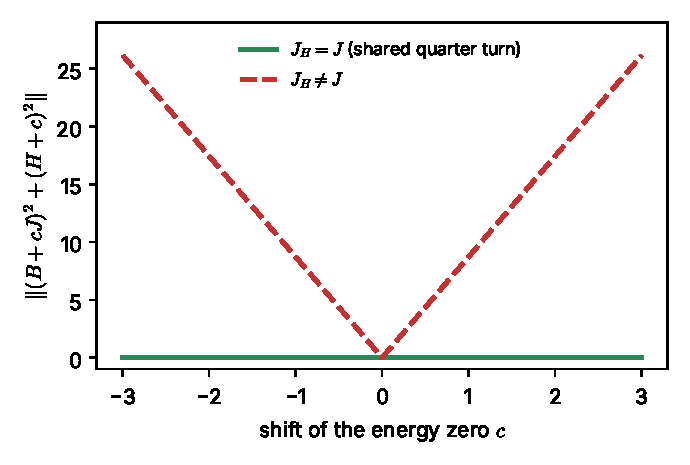
\includegraphics[width=0.6\textwidth]{figures/fig1-energy-zero.pdf}
\caption{The energy-zero argument on $\R^4$. Here $H$ has two doubly degenerate levels and $B=J_HH$ with $J_H$ commuting with $H$. Plotted is the violation of (A3), $\|(B+cJ)^2+(H+c\one)^2\|$, as the energy zero is shifted by $c$. When the shift is implemented by $J=J_H$ the violation is zero for all $c$; when it is implemented by a different complex structure $J\neq J_H$, it grows linearly in $|c|$.}
\label{fig:lever}
\end{figure}

\begin{remark}[A weaker form of (A4)]\label{rem:weak}
(A4) follows from the apparently weaker requirement that a shift of the energy zero changes the generator by an amount that depends on the shift but not on $H$, $A(H+c\one)=A(H)+f(c)$, with $f$ continuous. Indeed $f(c+c')=f(c)+f(c')$, so $f(c)=cF$; and since $0=\one-\one\in\mathcal{H}$, (A1) and (A3) give $A(0)^2=0$ with $A(0)$ antisymmetric, hence $A(0)=0$ and $F=A(\one)$.
\end{remark}

\begin{remark}[Why (A4) has content]
Without (A4), (A1)--(A3) hold for any antisymmetric generator with no kernel: given such an $A$, take $H=\hbar\sqrt{-A^2}$ and $J_H=A|A|^{-1}$, so that $A=J_HH/\hbar$ \cite{Aste,Vaughan}. Different Hamiltonians may then come with different complex structures. For example, on $\R^4$ let $J_0$ rotate the coordinate planes $(1,2)$ and $(3,4)$, let $P$ exchange the second and third basis vectors, and take $H_1=\mathrm{diag}(1,1,2,2)$ with $A(H_1)=J_0H_1/\hbar$ and $H_2=PH_1P^T$ with $A(H_2)=(PJ_0P^T)H_2/\hbar$. Each satisfies (A1)--(A3), but $PJ_0P^T$ rotates the planes $(1,3)$ and $(2,4)$, so the two complex structures differ. The polar construction also shows what goes wrong physically: it assigns each dynamics the Hamiltonian $\hbar\sqrt{-A^2}\ge0$, reading every energy as $|E|$ and reversing the sense of rotation of negative-energy levels. A real theory that reads its complex structure off each dynamics in this way makes the energy zero observable. (A4) is the requirement that it is not.
\end{remark}

\begin{proposition}[Antisymmetry from stability]\label{prop:stable}
Replace (A1) by the following two requirements, with $J:=\hbar A(\one)$:
\begin{itemize}
\item[(S)] \emph{Stability:} for every $H\in\mathcal{H}$, every solution of $\dot\psi=A(H)\psi$ stays bounded for all $t\in\R$.
\item[(T)] \emph{Completeness up to phase:} the only real matrices commuting with every observable are $a\one+bJ$, $a,b\in\R$.
\end{itemize}
Under (A0), (A3), (A4), (S) and (T), $J^T=-J$, $J^2=-\one$, and $A(H)=JH/\hbar$ with $[J,H]=0$ for every $H\in\mathcal{H}$. In particular (A1) and (A2) hold.
\end{proposition}

\begin{proof}
(A3) at $H=\one$ gives $J^2=-\one$. Steps (ii) and (iii) of the proof of Theorem~\ref{thm:main}, and the identities $JE+EJ=0$, $[E,H]=0$ and $E^2=0$ of step (iv), use only (A3), (A4) and $J^2=-\one$. So $[J,H]=0$ and $B=JH+E$, with $E^2=0$ and $E$ commuting with $H$. Let $\lambda$ be an eigenvalue of $H$ with eigenspace $V_\lambda$. $J$ and $E$ preserve $V_\lambda$, and $JH=\lambda J$ there. By (A4), $\hbar A(H-\lambda\one)=B-\lambda J$, which equals $E$ on $V_\lambda$. Since $E^2=0$, the flow of $A(H-\lambda\one)$ on $V_\lambda$ is $\one+tE/\hbar$, which is bounded only if $E=0$ on $V_\lambda$. By (S), $E=0$ on every eigenspace, so $E=0$ and $A(H)=JH/\hbar$. Finally, transposing $[J,H]=0$ for symmetric $H$ gives $[J^T,H]=0$, so by (A0) $J^T$ commutes with every observable, and by (T) $J^T=a\one+bJ$. Squaring, $(J^T)^2=(J^2)^T=-\one$ gives $(a^2-b^2+1)\one+2ab\,J=0$. Since $J$ is not a multiple of $\one$, $ab=0$ and $a^2-b^2=-1$, so $a=0$ and $b=\pm1$. $J^T=J$ is impossible, because a symmetric matrix has real eigenvalues and cannot square to $-\one$. Hence $J^T=-J$, and $(JH)^T=HJ^T=-JH$.
\end{proof}

(S) says that no state runs away under any of the dynamics. (T) holds in complex quantum theory, where the observables are the Hermitian matrices and the matrices commuting with all of them are the complex scalars $a+bi$. Norm preservation, the usual starting point, is therefore not needed as an assumption: given the energy-zero requirement and observables that determine states up to phase, the only stable dynamics are the norm-preserving ones. Without (S) the conclusion fails. On $\R^4$ with $J=J_0$, $H=\lambda\one$ and $B=\lambda J_0+E$, where $E=N\otimes\mathrm{diag}(1,-1)$ with $N=\left(\begin{smallmatrix}0&1\\0&0\end{smallmatrix}\right)$, so that $E^2=0$ and $E$ anticommutes with $J_0$, (A3) and (A4) hold at every shift, but $A(H-\lambda\one)=E/\hbar$ has the unbounded flow $\one+tE/\hbar$. With (S) in place of (A1), $A(0)=0$ still holds, since $A(0)^2=0$ and its flow is bounded. Remark~\ref{rem:weak} and Proposition~\ref{prop:shift} then go through, provided $c\mapsto A(H+c\one)$ is continuous, which replaces the bound $\|D(c)\|=|c|/\hbar$ used there.

\begin{proposition}[Planck--Einstein from the energy zero]\label{prop:pe}
Replace (A3) by
\begin{itemize}
\item[(A3$'$)] the rotation rate depends only on the energy: there is one function $g:\R\to\R$, with $|g|$ not constant, such that $A(H)^2=-g(H)^2$ for every $H\in\mathcal{H}$.
\end{itemize}
Under (A1), (A3$'$) and (A4) there are constants $\hbar>0$, $E_0$ and $\mu\ge0$ with $g(E)^2=[(E-E_0)^2+\mu^2]/\hbar^2$, and with $J:=\hbar A(\one)$ we have $J^T=-J$, $J^2=-\one$ and, for every $H\in\mathcal{H}$,
\begin{equation}\label{eq:gap}
A(H)=\frac{J(H-E_0\one)+M_H}{\hbar},\qquad [J,H]=[A(H),H]=0,
\end{equation}
where $M_H$ is antisymmetric, commutes with $H$, anticommutes with $J$ and satisfies $M_H^2=-\mu^2\one$. If some Hamiltonian has an energy eigenspace of real dimension $2$, then $\mu=0$ and $A(H)=J(H-E_0\one)/\hbar$ for every $H$: (A3) holds, with energies measured from $E_0$. Under (A0) and the maximality assumption (A5) of Section~\ref{sec:cons}, such a Hamiltonian always exists, and Proposition~\ref{prop:nogap} reaches $\mu=0$ instead from composition.
\end{proposition}

\begin{proof}
Since $\mathcal{H}$ contains $\one$ and is closed under shifts, $0\in\mathcal{H}$, and by (A4) $A(x\one)=Z+xK$ with $Z=A(0)$ and $K=A(\one)$. So $(Z+xK)^2=Z^2+x(ZK+KZ)+x^2K^2$ is a polynomial of degree at most two in $x$, and (A3$'$) at $H=x\one$ makes it equal to $-g(x)^2\one$. Hence $g(x)^2=\alpha x^2+\beta x+\gamma$ and $K^2=-\alpha\one$. By (A1) $K^2=-K^TK$, so $\alpha\ge0$, and $\alpha=0$ would give $K=0$, then $ZK+KZ=0$ and $g^2$ constant. So $\alpha>0$. Put $\hbar:=\alpha^{-1/2}$, $E_0:=-\beta/2\alpha$ and $\mu^2:=\hbar^2(\gamma-\alpha E_0^2)$, so that $g(E)^2=[(E-E_0)^2+\mu^2]/\hbar^2$. For any $H$, set $B:=\hbar A(H)$ and $H':=H-E_0\one$. Applying (A3$'$) to $H+c\one$ and comparing powers of $c$, as in step (ii) of the proof of Theorem~\ref{thm:main}, gives
\[
J^2=-\one,\qquad BJ+JB=-2H',\qquad B^2=-(H'^2+\mu^2\one).
\]
These differ from Eq.~\eqref{eq:coeffs} only by the constant $\mu^2$, which commutes with everything, and step (iii) goes through unchanged: $[J,H]=[B,H]=0$. Put $M_H:=B-JH'$. Then $JM_H+M_HJ=(JB+BJ)-2J^2H'=0$, $M_H$ commutes with $H$, and $B^2=(JH'+M_H)^2=-H'^2+(JH'M_H+M_HJH')+M_H^2=-H'^2+M_H^2$, since $M_HJH'=-JM_HH'=-JH'M_H$. So $M_H^2=-\mu^2\one$, and $\mu^2\ge0$ because $M_H$ is antisymmetric ($B$ by (A1), and $JH'$ because $J$ is antisymmetric and commutes with the symmetric $H'$). Let $V$ be an eigenspace of $H$ of real dimension $2$. $J$ and $M_H$ preserve $V$ and are antisymmetric there. On $\R^2$ every antisymmetric matrix is a multiple of the quarter turn, so $M_H|_V=tJ|_V$, and $JM_H+M_HJ=0$ gives $2tJ^2|_V=0$, so $M_H|_V=0$ and $\mu^2=0$. Under (A0) and (A5), any symmetric matrix commuting with $J$ whose complex eigenvalues on $\C^{n/2}$ are distinct is such a Hamiltonian.
\end{proof}

(A3$'$) says only that a state of definite energy $E$ turns at a rate $|g(E)|$ that is the same function of $E$ for every Hamiltonian. The energy-zero requirement then fixes the function. Its form, the linear law $\hbar\omega=|E-E_0|$, and the constant $\hbar$, read off as $g(E)^2\sim E^2/\hbar^2$ at large $E$, are outputs rather than inputs; $E_0$ is the energy at which nothing turns, the natural zero. The only alternative is a gap, $\hbar\omega=\sqrt{(E-E_0)^2+\mu^2}$, and it requires every energy level of every Hamiltonian to carry a second quarter turn $M_H/\mu$ anticommuting with $J$, a quaternionic structure. On $\R^8$, with $J=R_i$, $H$ commuting with $R_i$ and $R_j$, and $M_H=\mu R_j$, all of (A1), (A3$'$) and (A4) hold with $\mu\neq0$. A single non-degenerate level rules this out.

\section{Consequences for real and quaternionic quantum theory}\label{sec:cons}

\begin{corollary}\label{cor:real}
Real quantum theory, in which every symmetric matrix on $\R^n$ is an observable, cannot satisfy (A0)--(A4).
\end{corollary}

\begin{proof}
By (A0) and Theorem~\ref{thm:main}, $J$ commutes with every symmetric matrix. The only matrices commuting with all symmetric matrices are multiples of $\one$, and no multiple of $\one$ squares to $-\one$.
\end{proof}

\begin{remark}[Replacing (A0) by the energy zero]\label{rem:a0}
(A0) is used in two ways. In Corollary~\ref{cor:real}, Proposition~\ref{prop:complex} and Remarks~\ref{rem:quat} and~\ref{rem:a5} below, it is used only through its consequence
\begin{equation}\label{eq:JO}
[J,O]=0\quad\text{for every observable }O.
\end{equation}
In Proposition~\ref{prop:stable}, and in the last sentence of Proposition~\ref{prop:pe}, it is used to treat observables as Hamiltonians. For the first use, (A0) can be replaced by the requirement that only energy differences matter, stated for measurements rather than for generators:
\begin{itemize}
\item[(A0$'$)] Shifting the energy zero changes no measured average: for every $H\in\mathcal{H}$, every real $c$ and $t$, every state $\psi$ and every observable $O$, the average of $O$ in $e^{tA(H+c\one)}\psi$ equals its average in $e^{tA(H)}\psi$.
\end{itemize}
Under (A1), (A3) and (A4), (A0$'$) is equivalent to Eq.~\eqref{eq:JO}. By Theorem~\ref{thm:main}, $A(H+c\one)=A(H)+cJ/\hbar$ with $[J,A(H)]=0$, so $e^{tA(H+c\one)}\psi=R\chi$ with $\chi=e^{tA(H)}\psi$ and $R=e^{tcJ/\hbar}=\cos(tc/\hbar)\one+\sin(tc/\hbar)J$. As $\psi$ runs over all states so does $\chi$, and as $t$ and $c$ vary $R$ runs over all rotations $e^{sJ}$. So (A0$'$) says $\chi^TR^TOR\chi=\chi^TO\chi$ for all $\chi$ and all such $R$; since $R^TOR$ and $O$ are symmetric, this means $R^TOR=O$. At $s=\pi/2$, $R=J$, so $J^TOJ=O$, and with $J^T=-J$ and $J^2=-\one$ this gives $OJ=JO$. Conversely, if $OJ=JO$ then $(\cos s\,\one-\sin s\,J)O(\cos s\,\one+\sin s\,J)=(\cos^2s+\sin^2s)O=O$. (A0$'$) makes no claim about which operators generate dynamics, so it does not replace the second use of (A0); Proposition~\ref{prop:nogap} already removes the need for it in Proposition~\ref{prop:pe}, and Proposition~\ref{prop:stable} keeps (A0), because there antisymmetry of $J$ is what is being proved. Neither (A0) nor (A0$'$) can be dropped: real quantum theory with every symmetric matrix an observable, but with Hamiltonians restricted to those commuting with a fixed $J$ and $A(H)=JH/\hbar$, satisfies (A1)--(A4), and the average of any observable that does not commute with $J$ oscillates when the energy zero is shifted. With (A0$'$) in place of (A0), Corollary~\ref{cor:real} says that in real quantum theory with all symmetric observables the energy zero is measurable.
\end{remark}

Theorem~\ref{thm:main} together with (A0) places every observable in the set of symmetric matrices commuting with $J$. Identifying $(\R^n,J)$ with $\C^{n/2}$, with $J$ acting as multiplication by $i$, these are exactly the complex Hermitian matrices on $\C^{n/2}$. We add a maximality assumption:

\begin{itemize}
\item[(A5)] \emph{No superselection:} every symmetric matrix commuting with $J$ is an observable.
\end{itemize}

\begin{proposition}\label{prop:complex}
Under (A0)--(A5), the observables are exactly the complex Hermitian matrices on $\C^{n/2}$ and the dynamics is $\dot\psi=-\frac{i}{\hbar}H\psi$: the theory is complex quantum theory.
\end{proposition}

\begin{remark}[Quaternions]\label{rem:quat}
In quaternionic quantum theory \cite{Adler}, written over the reals, observables are the symmetric matrices commuting with the three anticommuting complex structures $R_i,R_j,R_k$ (right multiplication by $i,j,k$), and generators of dynamics are required to be quaternion-linear, i.e.\ to commute with $R_i,R_j,R_k$ as well. For two or more quaternionic levels, the real matrices commuting with every quaternionic Hermitian observable are spanned by $\one,R_i,R_j,R_k$, and the only quaternion-linear ones among them are multiples of $\one$. So no admissible $J$ exists and, by Theorem~\ref{thm:main} and (A0), quaternionic quantum theory violates (A4): in it, the energy zero is not a convention. If quaternion-linearity of the dynamics is dropped and $A(H)=R_iH/\hbar$ is used, (A0)--(A4) hold with $J=R_i$, but (A5) fails: a quaternionic two-level system on $\R^8$ has $6$ independent observables, while $16$ symmetric matrices commute with $J$. Restoring them gives complex quantum theory.
\end{remark}
\begin{remark}[What (A5) excludes]\label{rem:a5}
(A5) is an independent assumption. By Theorem~\ref{thm:main} and Eq.~\eqref{eq:JO} the observables are some set of complex Hermitian matrices containing $\one$; (A5) asks for all of them, and we read it as the absence of superselection rules. Three smaller sets show what it excludes. In each, take $\mathcal{H}$ to be the set of observables and $A(H)=JH/\hbar$, so that (A0)--(A4) and (S) hold.
(i) \emph{Superselection:} the Hermitian matrices commuting with a projector $P\neq0,\one$ that commutes with $J$. The real matrices commuting with all of them include $P$ and $JP$, so (T) fails.
(ii) \emph{Quaternionic observables} with $J=R_i$, as in the previous remark. The real matrices commuting with all of them are spanned by $\one,R_i,R_j,R_k$, so (T) fails.
(iii) \emph{A spin factor:} on $\C^8$, let $\gamma_1,\dots,\gamma_7$ be Hermitian with $\gamma_a\gamma_b+\gamma_b\gamma_a=2\delta_{ab}\one$, and let the observables be the real span of $\one,\gamma_1,\dots,\gamma_7$: $8$ observables, where (A5) asks for the $64$ Hermitian matrices on $\C^8$. The set is closed under the Jordan product $O\circ O'=\frac12(OO'+O'O)$, and the only real matrices commuting with all of it are $a\one+bJ$, so (T) holds too. (A6), (A7) and (C) constrain the dynamics and the joint state space but not the joint observables, so the composites of Section~\ref{sec:comp} do not exclude it either. A requirement on joint observables does: if they are spanned by products of local observables (local tomography) and closed under the Jordan product, then $(\gamma_1\otimes\gamma_1)\circ(\gamma_2\otimes\gamma_2)=(\gamma_1\gamma_2)\otimes(\gamma_1\gamma_2)$ must lie in that span, and it does not. Barnum and Wilce prove the general statement: Jordan-algebraic systems with locally tomographic composites, at least one of them a complex qubit, are complex quantum systems up to superselection rules \cite{BarnumWilce}, and (T) removes those. Deriving (A5) in this way replaces one assumption by several (Jordan closure, (T), local tomography with Jordan-closed joint observables, and a qubit), so we keep (A5).
\end{remark}

\section{Composite systems}\label{sec:comp}

Consider two systems with state spaces $\R^{n_A},\R^{n_B}$ and complex structures $J_A,J_B$ given by Theorem~\ref{thm:main}. Let the joint state space $W$ be a subspace of $\R^{n_A}\otimes\R^{n_B}$, and assume:

\begin{itemize}
\item[(A6)] The joint system satisfies (A1)--(A4) with its own complex structure $J_{AB}$, and for non-interacting subsystems a Hamiltonian of $A$ alone, $H_A\otimes\one$, generates $A(H_A)\otimes\one$ on $W$ (and likewise for $B$).
\item[(A7)] $W$ is the largest subspace of $\R^{n_A}\otimes\R^{n_B}$ compatible with (A6).
\end{itemize}
A joint space built as a quotient of $\R^{n_A}\otimes\R^{n_B}$, as in Ref.~\cite{BarriosHita}, is covered by identifying the quotient with the orthogonal complement of the kernel.

\begin{proposition}\label{prop:composite}
Under (A6), $J_A\otimes\one=\one\otimes J_B=J_{AB}$ on $W$. Under (A7), $W$ is the $(-1)$-eigenspace of $J_A\otimes J_B$, of real dimension $n_An_B/2$. With $J_{AB}$ as its complex structure, it is the complex tensor product $\C^{n_A/2}\otimes_{\C}\C^{n_B/2}$, on which $J_A\otimes J_B=-\one$, and if (A5) holds for $A$, $B$ and the joint system, products of local observables span all joint observables (local tomography).
\end{proposition}

\begin{proof}
A constant shift of the total energy, $c\one_{AB}$, can be written as $(c\one_A)\otimes\one_B$ or as $\one_A\otimes(c\one_B)$. By (A6) and Theorem~\ref{thm:main} for the subsystems, these shifts change the joint generator by $c(J_A\otimes\one)/\hbar$ and by $c(\one\otimes J_B)/\hbar$ respectively, while Theorem~\ref{thm:main} for the joint system says both changes equal $cJ_{AB}/\hbar$. Hence $J_A\otimes\one=\one\otimes J_B=J_{AB}$ on $W$.

The operators $J_A\otimes\one$ and $\one\otimes J_B$ commute and square to $-\one$, so $K:=J_A\otimes J_B=(J_A\otimes\one)(\one\otimes J_B)$ is a symmetric involution with $\tr K=(\tr J_A)(\tr J_B)=0$. If $(J_A\otimes\one)v=(\one\otimes J_B)v$, then $Kv=(J_A\otimes\one)^2v=-v$. Conversely, if $Kv=-v$, then applying $J_A\otimes\one$ gives $-(\one\otimes J_B)v=-(J_A\otimes\one)v$. So the largest $W$ is the $(-1)$-eigenspace of $K$, of dimension $n_An_B/2$. Under the identification of $(\R^{n_X},J_X)$ with $\C^{n_X/2}$, the real tensor product decomposes as $(\C^{n_A/2}\otimes_\C\C^{n_B/2})\oplus(\C^{n_A/2}\otimes_\C\overline{\C^{n_B/2}})$, with $K=-\one$ on the first summand and $K=+\one$ on the second. Local dynamics $(J_AH_A)\otimes\one$ commutes with $K$ and so preserves $W$. On the complex tensor product, products of Hermitian matrices on the factors span all Hermitian matrices on the product, which is local tomography \cite{Hardy,MasanesMuller}.
\end{proof}

\paragraph{(A4) from composition.} The first step of the proof above uses only that a constant shift of the total energy can be booked to either subsystem. That fact alone yields (A4) for each subsystem, without assuming it. We need:
\begin{itemize}
\item[(C)] For non-interacting subsystems, the joint generator depends only on the joint Hamiltonian and is the sum of the subsystem generators, $A_{AB}(H_A\otimes\one+\one\otimes H_B)=A_A(H_A)\otimes\one+\one\otimes A_B(H_B)$ on $W$; and local operators act faithfully on $W$: if $X\otimes\one=Y\otimes\one$ on $W$, then $X=Y$.
\end{itemize}

\begin{proposition}\label{prop:shift}
Let a system $A$ satisfy (A1) and (A3), and let it have a partner system $B$, for instance a copy of $A$, with which (C) holds. Then $A$ satisfies (A4).
\end{proposition}

\begin{proof}
For real $c$ put $D_{H}(c):=A_A(H+c\one)-A_A(H)$, and define $D'_{H_B}(c)$ in the same way for $B$. The operators $(H_A+c\one)\otimes\one+\one\otimes H_B$ and $H_A\otimes\one+\one\otimes(H_B+c\one)$ are equal, so by (C) they have the same joint generator, and $D_{H_A}(c)\otimes\one=\one\otimes D'_{H_B}(c)$ on $W$. The right side does not depend on $H_A$, so by faithfulness $D(c):=D_{H_A}(c)$ is the same for every $H_A$. Then $D(c+c')=[A_A(H+(c+c')\one)-A_A(H+c\one)]+D(c)=D(c')+D(c)$. Since $0\in\mathcal{H}$, (A1) and (A3) give $A_A(0)=0$ as in Remark~\ref{rem:weak}, so $D(c)=A_A(c\one)$ is antisymmetric with $D(c)^2=-c^2\one/\hbar^2$. Hence $D(c)^TD(c)=c^2\one/\hbar^2$ and $\|D(c)\|=|c|/\hbar$. An additive map bounded near $0$ is linear, so $D(c)=c\,D(1)=c\,A_A(\one)$, which is (A4).
\end{proof}

Faithfulness holds on the full real tensor product, and also on the balanced product of Proposition~\ref{prop:composite}. That $W$ contains $u\otimes v-J_Au\otimes J_Bv$ for all $u,v$; if $X\otimes\one$ annihilates these vectors, then $Xu\otimes v=XJ_Au\otimes J_Bv$, and since $v$ and $J_Bv$ are linearly independent, $Xu=0$ for every $u$. So the energy-zero requirement need not be postulated. It follows from requiring that the dynamics of a composite be fixed by its total Hamiltonian, with non-interacting parts evolving independently: a constant in the total energy cannot be assigned to either part. Theorem~\ref{thm:main} turns this into one complex structure for each system, and the same booking argument gives $J_A\otimes\one=\one\otimes J_B$. Proposition~\ref{prop:rp} below gives a second, independent route to (A4) for theories with a Euclidean formulation.

Composition also settles the one case left open by Proposition~\ref{prop:pe}, and fixes $\hbar$ across systems.

\begin{proposition}[No gap for composites]\label{prop:nogap}
Let systems $A$ and $B$ each satisfy (A1), (A3$'$) and (A4), with $\hbar_A,\mu_A,J_A$ and $\hbar_B,\mu_B,J_B$ as in Proposition~\ref{prop:pe} (the functions $g_A,g_B$ may differ). Let $W$ be the balanced product, the subspace of $\R^{n_A}\otimes\R^{n_B}$ on which $J_A\otimes\one=\one\otimes J_B$, and let (C) hold on $W$. Then $\hbar_A=\hbar_B$ and $\mu_A=\mu_B=0$, so both systems satisfy (A3) with energies measured from their own $E_0$.
\end{proposition}

\begin{proof}
Write $P=J_A\otimes\one$ and $Q=\one\otimes J_B$. They commute, square to $-\one$, and $W$ is where $Pw=Qw$. Booking a constant to either part, as in the proof of Proposition~\ref{prop:shift}, gives $cP/\hbar_A=cQ/\hbar_B$ on $W$, so $\hbar_A=\hbar_B$. By Eq.~\eqref{eq:gap}, $\hbar A_A(H_A)\otimes\one+\one\otimes\hbar A_B(H_B)=S_J+X+Y$ with $S_J=J_AH_A'\otimes\one+\one\otimes J_BH_B'$, $H'=H-E_0\one$ on each side, $X=M_{H_A}\otimes\one$ and $Y=\one\otimes M_{H_B}$. $S_J$ commutes with $P$ and $Q$ and so maps $W$ into $W$; by (C) the joint generator acts on $W$, so $X+Y$ maps $W$ into $W$. But $X$ anticommutes with $P$ and commutes with $Q$, so for $w\in W$, $PXw=-XPw=-XQw=-QXw$: $X$ sends $W$ into the subspace where $P=-Q$, and so does $Y$. Hence $Q(X+Y)w=P(X+Y)w=-Q(X+Y)w$, and $(X+Y)w=0$ on $W$. Since $P$ maps $W$ into $W$, also $(X+Y)Pw=0$, so $XPw=-YPw=-PYw=PXw$, while $XPw=-PXw$. So $PXw=0$, hence $Xw=0$: $M_{H_A}\otimes\one$ vanishes on $W$, and by faithfulness $M_{H_A}=0$. So $\mu_A=0$, and likewise $\mu_B=0$.
\end{proof}

(A3$'$) itself is not a consequence of composition. Two rules satisfy (A1), (A2), (A4) and (C) on the complex tensor product but not (A3$'$): $A(H)=-\frac{i}{\hbar}\bigl(H+\kappa\,\textstyle\sum_\lambda P_\lambda QP_\lambda\bigr)$, where $P_\lambda$ are the eigenprojections of $H$ and $Q$ is a fixed additive charge, so that a state turns at a rate set by its energy plus $\kappa$ times its charge; and $A(H)=-\frac{i}{\hbar}\bigl((1+\kappa)H-\kappa\langle H\rangle\one\bigr)$, with $\langle H\rangle=\mathrm{tr}H/n$ the mean energy, so that a state's rate depends on the rest of the spectrum. The content of (A3$'$) is therefore that a state's rate is set by its own energy alone.

Without (A6), on the full real tensor product $J_A\otimes\one\neq\one\otimes J_B$, and $J_A\otimes J_B$ is a joint observable invisible to local measurements, the extra parameter responsible for the failure of local tomography in real quantum theory and probed in Refs.~\cite{Renou,Chen,Li}. Figure~\ref{fig:counts} compares the counts for two two-level systems. Proposition~\ref{prop:composite} recovers the ``balanced tensor product'' identified by Bang, Cho and Baek in recent real formulations \cite{BangChoBaek}, here as a consequence of the energy-zero requirement.

\begin{figure}[t]
\centering
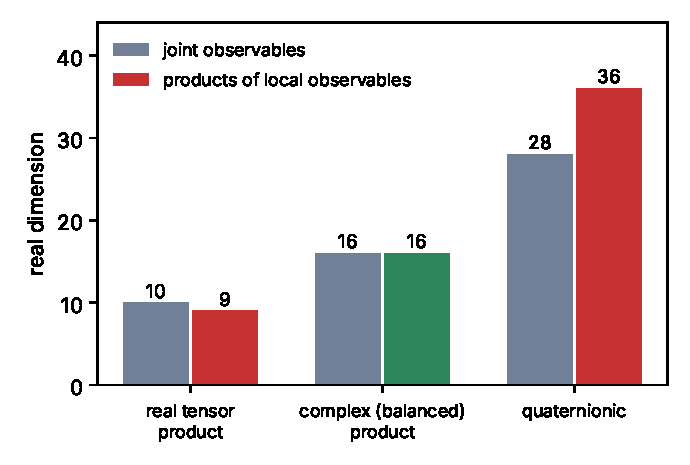
\includegraphics[width=0.6\textwidth]{figures/fig2-local-tomography.pdf}
\caption{Real dimension of the joint observables compared with the span of products of local observables, for two two-level systems. Real tensor product: $10$ joint versus $9$ local (one joint parameter is invisible locally). Complex (balanced) product: $16$ and $16$. Quaternionic: $28$ joint quaternionic Hermitian observables versus $6\times6=36$ products, so the local products cannot all be joint observables.}
\label{fig:counts}
\end{figure}

\section{The recent real formulations}\label{sec:real}

Three recent proposals reproduce all predictions of complex quantum theory, including the network predictions of Ref.~\cite{Renou}, using real matrices: Hoffreumon and Woods \cite{HoffreumonWoods}, Barrios Hita \emph{et al.} \cite{BarriosHita}, and Maioli, Curado and Gazeau \cite{MaioliCuradoGazeau}. We test each against (A0)--(A7), using the definitions as each paper states them. None of the three defines a Hamiltonian flow; each maps unitaries to real orthogonal (and, where stated, symplectic) matrices, and we take the dynamics to be the image of the complex one, $e^{-iHt}\mapsto\exp(-tJ\,\Gamma(H))$, where $\Gamma$ is the paper's map from complex to real matrices and $J=\Gamma(i\one)$.

\begin{itemize}
\item \emph{Hoffreumon--Woods.} Observables are $\Gamma(H)=\one\otimes\operatorname{Re}H+J\otimes\operatorname{Im}H$, and their Lemma~B.6 characterizes the image as exactly the symmetric matrices commuting with $J_n=J\otimes\one$. So (A5) holds with the shared $J=J_n$. Their composition rule (their Eq.~B.34), $\Gamma(M_1)\boxtimes\Gamma(M_2)=\tfrac12[\Gamma(M_1)\otimes\Gamma(M_2)-\Gamma(iM_1)\otimes\Gamma(iM_2)]$, equals $\Pi\,(\Gamma(M_1)\otimes\Gamma(M_2))$ with $\Pi=\tfrac12(\one-J_n\otimes J_n)$, since $\Gamma(iM)=J_n\Gamma(M)$. $\Pi$ is the projector onto the $(-1)$-eigenspace of $J_n\otimes J_n$, which is the space $W$ of Proposition~\ref{prop:composite}.
\item \emph{Barrios Hita et al.} Each system lives on $\R^d\otimes\R^2_F$, and observables have the form $\operatorname{Re}\Pi\otimes\one+\operatorname{Im}\Pi\otimes J_F$, which are exactly the symmetric matrices commuting with $J=\one\otimes J_F$. Their composite is the quotient of the real tensor product by a kernel spanned, on each pair of flags, by $|00\rangle+|11\rangle$ and $|01\rangle-|10\rangle$. This kernel is the $(+1)$-eigenspace of $J\otimes J$, so the quotient is $W$. This is the balanced tensor product identified by Bang, Cho and Baek \cite{BangChoBaek}.
\item \emph{Maioli--Curado--Gazeau.} Their map is $\gamma^{-1}(L)=\one\otimes\operatorname{Re}L+\tau\otimes\operatorname{Im}L$, with multiplication by $i$ represented by $J=\tau\otimes\one$, $\tau^2=-\one$. Their composition rule is $L_A\otimes_K L_B=\gamma^{-1}(\gamma(L_A)\otimes_{\C}\gamma(L_B))$, the real form of the complex tensor product, which commutes with $J$.
\end{itemize}

In all three, (A1)--(A4) hold with the stated dynamics, (A5) holds, and the composite is exactly $W$, so (A6) and (A7) hold. Each therefore carries, explicitly, one complex structure $J$ commuting with every observable and every generator and shared by subsystems through $J\otimes\one=\one\otimes J$. Theorem~\ref{thm:main} and Proposition~\ref{prop:composite} explain why: these features are not choices made by the authors but are forced by the conventionality of the energy zero. Conversely, the one real theory that lacks a shared $J$, real quantum theory with all symmetric observables and the plain tensor product, is the theory ruled out experimentally \cite{Renou,Chen,Li}, and by Corollary~\ref{cor:real} it is also the one in which the energy zero is observable. Each claim in this section was checked numerically against the papers' stated formulas (Appendix).

\section{Euclidean formulations and reflection positivity}\label{sec:rp}

Assumption (A4) can be motivated from the Euclidean side. Suppose the dynamics of each $H\in\mathcal{H}$ comes from a Euclidean theory, a positive real semigroup $e^{-\tau H}$, by Osterwalder--Schrader reconstruction and continuation $\tau\to it$ \cite{OS1,OS2}. We show that every theory obtained this way satisfies (A1)--(A4). (A4) then holds automatically for any theory with a Euclidean formulation.

\paragraph{Reflection positivity for a transfer matrix.}
Let $T$ be a real $n\times n$ matrix, and give a path $x_0\to x_1\to\dots\to x_N$ in $\{1,\dots,n\}$ the weight $\prod_j T_{x_{j+1}x_j}$. Let $\theta$ reverse time, $x_j\mapsto x_{N-j}$, with complex conjugation on functionals, and let $\mathcal{A}_+$ be the functionals of the later half of the path. Reflection positivity is $\langle\theta F,F\rangle\ge 0$ for all $F\in\mathcal{A}_+$. For reflection through a site ($N$ even) it holds if and only if $T$ is symmetric, since then $\langle\theta F,F\rangle=\sum_x|g_F(x)|^2$. For reflection through a link ($N$ odd) it holds if and only if, in addition, $T\ge 0$, since then $\langle\theta F,F\rangle=g_F^{T}Tg_F$. This is the standard transfer-matrix criterion \cite{OsterwalderSeiler,FILS,GlimmJaffe}. For $T=\one-\epsilon H/\hbar$ it holds for small $\epsilon$ whenever $H$ is symmetric. For the implicit step $T=(\one+\epsilon H/\hbar)^{-1}$ it holds at every $\epsilon>0$ if and only if $H\ge0$. In either case, reconstruction gives the real Hilbert space $\R^n$ and the semigroup $e^{-\tau H/\hbar}$. With a complex weight $T=\one+z\epsilon H$, reflection positivity fails for every $z\notin\R$ and every $H\neq 0$. The simplest pairing is then $(z\epsilon H_{12})^2$, which is not real, and at $z=-i/\hbar$ it is negative. In real time the role of positivity is taken over by unitarity.

\begin{proposition}\label{prop:rp}
Let $\mathcal{H}$ be a set of real symmetric $n\times n$ matrices containing $\one$ and closed under $H\mapsto H+c\one$. Define the real-time dynamics of each $H$ by continuing its Euclidean semigroup, $e^{-\tau H/\hbar}\mapsto e^{-itH/\hbar}$, on the complexification $\C^n\cong\R^{2n}$. Written over the reals, with $i$ represented by $J=\begin{pmatrix}0&-\one\\ \one&0\end{pmatrix}$ and $H$ acting as $H\oplus H$, the generator is $A(H)=-J(H\oplus H)/\hbar$. It satisfies (A1)--(A4) with the single complex structure $-J$.
\end{proposition}

\begin{proof}
$J$ is antisymmetric, squares to $-\one$ and commutes with $H\oplus H$, so $A(H)$ is antisymmetric (A1) and commutes with $H\oplus H$ (A2), and $A(H)^2=J^2(H\oplus H)^2/\hbar^2=-(H\oplus H)^2/\hbar^2$ (A3). The continuation acts on the time parameter, not on $H$, so $A(H)$ is linear in $H$ with one coefficient $-J/\hbar$, and $A(H+c\one)=A(H)+cA(\one)$ (A4).
\end{proof}

The content of the proposition is in the last step. On the Euclidean side, a shift of the energy zero multiplies every path weight by the same positive number $e^{-c\tau/\hbar}$, for every $H$. That is trivially a convention there. The continuation carries this common positive factor to a common rotation $e^{-ict/\hbar}$, which is (A4). The imaginary unit is needed exactly at the continuation, since $e^{-itH/\hbar}$ is real for all $t$ only if $H=0$. It enters as one scalar, the same for every $H$.

\begin{corollary}\label{cor:rp}
Real quantum theory in which every symmetric matrix is an observable and a Hamiltonian is not the continuation of any family of reflection-positive Euclidean theories.
\end{corollary}

\begin{proof}
By Proposition~\ref{prop:rp} such a continuation satisfies (A1)--(A4). By Corollary~\ref{cor:real} real quantum theory does not.
\end{proof}

Theorem~\ref{thm:main} therefore applies to every theory with a reflection-positive Euclidean formulation, and the shared $J$ it produces is the imaginary unit of the Wick rotation. The scope is that of the rest of the paper: finite-dimensional state spaces with given Hamiltonians. For field theories the proposition applies whenever a reflection-positive Euclidean measure exists, but constructing such a measure is the hard part of constructive field theory, and we do not address it here. We have not found this link between reflection positivity and the energy-zero requirement stated in the literature we reviewed. The step is short, and we would welcome references.

\section{Relation to prior work}

That an energy-conserving, norm-preserving real dynamics carries a complex structure is known: the positive-frequency complex structure of Ashtekar and Magnon \cite{AshtekarMagnon}, discussed for finite-dimensional real quantum theory by Aste \cite{Aste} and Vaughan \cite{Vaughan}; Gibbons and Pohle note that a Hamiltonian picks out a complex structure \cite{GibbonsPohle}. These results give a $J$ per dynamics and, as Vaughan notes, do not exclude quaternions. Myrheim's real-Hilbert-space formulation imposes $[J,H]=0$ rather than deriving it \cite{Myrheim}. In the convex-operational setting, the link between observables and generators of dynamics is known to single out complex quantum theory. Alfsen and Shultz characterize the self-adjoint parts of C$^*$-algebras among Jordan algebras by a dynamical correspondence, a linear map from observables to generators under which each observable is conserved by its own dynamics and which satisfies a commutator condition \cite{AlfsenShultz}; Niestegge extends this to a wider class of algebras \cite{Niestegge}; and Barnum, M\"uller and Ududec derive complex quantum theory from the requirement that energy be observable, meaning that every generator of reversible dynamics is assigned, injectively and linearly, an observable it conserves \cite{BMU}. These results assume a linear correspondence on all observables, or on the whole Lie algebra of dynamics, within a Jordan-algebraic framework. Theorem~\ref{thm:main} assumes linearity only in the direction of $\one$, that is, for shifts of the energy zero, together with the spectral condition (A3), and derives $A(H)=JH/\hbar$ on a real Hilbert space. Barnum and Wilce show that local tomography singles out complex quantum theory among Jordan-algebraic theories \cite{BarnumWilce}; Proposition~\ref{prop:composite} reaches the complex tensor product from the energy-zero requirement instead, without a Jordan-algebraic framework. A universal $J$ commuting with all observables was postulated by Stueckelberg \cite{Stueckelberg} and derived from Poincar\'e symmetry for elementary relativistic systems by Moretti and Oppio \cite{MorettiOppio}. The present argument instead uses only time translations together with the freedom to shift the energy zero, and does not require relativistic symmetry. We have not found the energy-zero argument of Theorem~\ref{thm:main}, or its use for composites in Proposition~\ref{prop:composite}, in the literature we reviewed, but we would welcome references.

\section{Discussion}

Rotation alone does not force complex numbers: every rotation dynamics has a quarter turn of its own. What forces a single imaginary unit is the requirement that the zero of energy be a convention. In real quantum theory with all symmetric observables, shifting the energy zero would be observable, since no quarter turn commutes with every observable. Section~\ref{sec:real} makes the status of the recent debate \cite{HoffreumonWoods,BarriosHita,MaioliCuradoGazeau,BangChoBaek,FengRenVedral} precise. Every real formulation that matches experiment, as stated by its authors, satisfies (A0)--(A7) and contains the shared $J$ and the complex tensor product. Whether such a theory should be called ``real'' is then a question of terminology. The physical content, a single complex structure shared by all dynamics and all subsystems, is not optional.

The assumptions can be weakened in obvious directions (infinite dimensions, unbounded Hamiltonians) that we do not pursue here. (A4) is the load-bearing assumption. It says the shift of the energy zero acts as $c\,A(\one)$, the same common rotation for every $H$. It is not an extra postulate. Proposition~\ref{prop:shift} derives it from the consistency of composite systems, and for theories with a reflection-positive Euclidean formulation Proposition~\ref{prop:rp} shows that the Wick rotation supplies it, with the rotation's own imaginary unit as the shared $J$. What remains are the requirement that the rotation rate of an energy eigenstate depend only on its own energy, from which Propositions~\ref{prop:pe} and~\ref{prop:nogap} recover the Planck--Einstein relation (A3) and a single $\hbar$, and which composition alone does not supply, the requirement that non-interacting systems evolve independently, either norm preservation (A1) or, by Proposition~\ref{prop:stable}, stability of every dynamics together with completeness of the observables up to the common phase, and, for the conclusions about observables, (A0$'$), which is (A4) read as a statement about measured averages (Remark~\ref{rem:a0}). The maximality assumption (A5), used only to identify the observables with all complex Hermitian matrices, is independent of the others: Remark~\ref{rem:a5} gives a spin-factor theory that meets every other assumption, and excluding it needs further assumptions on joint observables.

\section*{Acknowledgments}
[To confirm before submitting: The author used an AI assistant for literature search, symbolic and numerical checks, and drafting. The author has checked every step and every reference and takes full responsibility for the content.]

\appendix
\section{Checks}
Each step was verified with a short script (supplied as an ancillary file, \texttt{anc/checks.py}). It checks, in exact arithmetic with SymPy and numerically with NumPy: that complex quantum theory satisfies (A1)--(A4); the polar complex structure of a single dynamics and the counterexample in the Remark after Theorem~\ref{thm:main}; the unique solution $B=JH$ on $\R^4$ for generic and degenerate $H$, with the antisymmetric part forced to zero; that the commutant of all symmetric matrices is one-dimensional; the quaternionic counts, and that no quaternion-linear $J$ commutes with all quaternionic observables; the dimension and local-tomography counts of Proposition~\ref{prop:composite} for $1\times1$, $2\times2$ and $2\times3$ complex levels; and, for Section~\ref{sec:real}, that the observables of Refs.~\cite{HoffreumonWoods,BarriosHita} are exactly the symmetric matrices commuting with their $J$, that the image of $e^{-iHt}$ is $\exp(-tJ\Gamma(H))$, that the Hoffreumon--Woods product equals $\Pi(\Gamma(M_1)\otimes\Gamma(M_2))$ and restricts on $W$ to the complex tensor product, that the Barrios Hita kernel is the $(+1)$-eigenspace of $J\otimes J$, and that the Maioli--Curado--Gazeau rule is the real form of the complex tensor product commuting with $J$; and that steps (ii)--(iii) of the proof force $[J,H]=0$ and $[B,H]=0$ for any $J$ with $J^2=-\one$; and, for Proposition~\ref{prop:shift}, that the two bookings of a constant give the same joint Hamiltonian, that an $H$-dependent shift rotation would give two different joint generators for it, and that local operators act faithfully on the balanced product; and, for Proposition~\ref{prop:stable}, the nilpotent counterexample that satisfies (A3) and (A4) but not (S), and that a complex structure that is not orthogonal leaves too few observables for (T); and, for Proposition~\ref{prop:pe}, that $(Z+xK)^2$ is quadratic in $x$, that $A(H)=J(H-E_0\one)/\hbar$ satisfies (A3$'$) at every shift, the gapped example on $\R^8$ with frequencies $\sqrt{(E-E_0)^2+\mu^2}/\hbar$, and that on a level of real dimension $2$ no nonzero antisymmetric matrix anticommutes with $J$; for Proposition~\ref{prop:nogap}, that on $\R^4\otimes\R^4$ with $J=R_i$ each gap term sends the balanced product into the subspace where $P=-Q$ and only $M_A=M_B=0$ keeps the joint generator on $W$; and the two rules that satisfy everything but (A3$'$); and, for Remark~\ref{rem:a0}, that real quantum theory with only $J$-commuting Hamiltonians satisfies (A1)--(A4) while a shift of the energy zero changes the average of an observable not commuting with $J$, and that invariance under $J$ alone separates observables that commute with $J$ from those that do not; and, for Remark~\ref{rem:a5}, that the superselected and quaternionic observable sets leave a commutant of dimension $4$, while the spin factor on $\C^8$ is Jordan-closed, has commutant spanned by $\one$ and $J$, and fails Jordan closure of the span of local products. All 29 checks pass. Steps (ii)--(iv) of the proof, including the derivation of (A2), are also checked in Lean~4 over an arbitrary ring without 2-torsion (ancillary file \texttt{anc/EnergyShift.lean}), and the booking argument of Proposition~\ref{prop:shift}, that $D(c)$ is independent of $H$ and additive, is checked in \texttt{anc/Booking.lean}, the algebraic steps of Proposition~\ref{prop:stable} in \texttt{anc/Stability.lean}, and those of Proposition~\ref{prop:pe}, that $[J,H]=[B,H]=0$, $JM_H+M_HJ=0$ and $M_H^2=-\mu^2\one$, in \texttt{anc/PlanckEinstein.lean}, and the proof of Proposition~\ref{prop:nogap}, that the gap terms vanish on $W$, in \texttt{anc/NoGap.lean}, and the two directions of the equivalence in Remark~\ref{rem:a0}, $J^TOJ=O\Rightarrow[J,O]=0$ and $[J,O]=0\Rightarrow R^TOR=O$, in \texttt{anc/Unseen.lean}.

\begin{thebibliography}{99}
\bibitem{AshtekarMagnon} A.~Ashtekar and A.~Magnon, ``Quantum fields in curved space-times,'' Proc.\ R.\ Soc.\ Lond.\ A \textbf{346}, 375 (1975).
\bibitem{Aste} A.~Aste, ``Origin of the complex structure of quantum mechanics,'' arXiv:1905.12894 (2019).
\bibitem{Vaughan} M.~P.~Vaughan, ``The requirement of (at least) complex structure for quantum mechanics,'' arXiv:2609.23041 (2026).
\bibitem{Stueckelberg} E.~C.~G.~Stueckelberg, ``Quantum theory in real Hilbert space,'' Helv.\ Phys.\ Acta \textbf{33}, 727 (1960).
\bibitem{MorettiOppio} V.~Moretti and M.~Oppio, ``Quantum theory in real Hilbert space: How the complex Hilbert space structure emerges from Poincar\'e symmetry,'' arXiv:1611.09029.
\bibitem{Renou} M.-O.~Renou \emph{et al.}, ``Quantum theory based on real numbers can be experimentally falsified,'' Nature \textbf{600}, 625 (2021).
\bibitem{Chen} M.-C.~Chen \emph{et al.}, ``Ruling out real-valued standard formalism of quantum theory,'' Phys.\ Rev.\ Lett.\ \textbf{128}, 040403 (2022).
\bibitem{Li} Z.-D.~Li \emph{et al.}, ``Testing real quantum theory in an optical quantum network,'' Phys.\ Rev.\ Lett.\ \textbf{128}, 040402 (2022).
\bibitem{HoffreumonWoods} T.~Hoffreumon and M.~P.~Woods, ``Quantum theory does not need complex numbers,'' arXiv:2504.02808 (2025).
\bibitem{BarriosHita} P.~Barrios Hita, A.~Trushechkin, H.~Kampermann, M.~Epping and D.~Bru\ss, ``Quantum mechanics based on real numbers: A consistent description,'' Phys.\ Rev.\ Lett.\ \textbf{136}, 240202 (2026); arXiv:2503.17307.
\bibitem{MaioliCuradoGazeau} A.~C.~Maioli, E.~M.~F.~Curado and J.-P.~Gazeau, ``Quantum mechanics over real numbers fully reproduces standard quantum theory,'' arXiv:2604.19482 (2026).
\bibitem{BangChoBaek} J.~Bang, K.~Cho and K.~Baek, ``Hidden complex structure in quotient-space real quantum mechanics,'' arXiv:2607.05865 (2026).
\bibitem{FengRenVedral} T.~Feng, C.~Ren and V.~Vedral, ``Locality implies complex numbers in quantum mechanics,'' arXiv:2504.07808 (2025).
\bibitem{GibbonsPohle} G.~W.~Gibbons and H.-J.~Pohle, ``Complex numbers, quantum mechanics and the beginning of time,'' arXiv:gr-qc/9302002 (1993).
\bibitem{Myrheim} J.~Myrheim, ``Quantum mechanics on a real Hilbert space,'' arXiv:quant-ph/9905037 (1999).
\bibitem{AlfsenShultz} E.~M.~Alfsen and F.~W.~Shultz, ``On orientation and dynamics in operator algebras. Part I,'' Commun.\ Math.\ Phys.\ \textbf{194}, 87 (1998).
\bibitem{Niestegge} G.~Niestegge, ``Dynamical correspondence in a generalized quantum theory,'' Found.\ Phys.\ (2015), doi:10.1007/s10701-015-9881-x; arXiv:1402.0158.
\bibitem{BMU} H.~Barnum, M.~P.~M\"uller and C.~Ududec, ``Higher-order interference and single-system postulates characterizing quantum theory,'' New J.\ Phys.\ \textbf{16}, 123029 (2014); arXiv:1403.4147.
\bibitem{BarnumWilce} H.~Barnum and A.~Wilce, ``Local tomography and the Jordan structure of quantum theory,'' Found.\ Phys.\ \textbf{44}, 192 (2014); arXiv:1202.4513.
\bibitem{Adler} S.~L.~Adler, \emph{Quaternionic Quantum Mechanics and Quantum Fields} (Oxford University Press, 1995).
\bibitem{Hardy} L.~Hardy, ``Quantum theory from five reasonable axioms,'' arXiv:quant-ph/0101012 (2001).
\bibitem{MasanesMuller} Ll.~Masanes and M.~P.~M\"uller, ``A derivation of quantum theory from physical requirements,'' New J.\ Phys.\ \textbf{13}, 063001 (2011).
\bibitem{OS1} K.~Osterwalder and R.~Schrader, ``Axioms for Euclidean Green's functions,'' Commun.\ Math.\ Phys.\ \textbf{31}, 83 (1973).
\bibitem{OS2} K.~Osterwalder and R.~Schrader, ``Axioms for Euclidean Green's functions II,'' Commun.\ Math.\ Phys.\ \textbf{42}, 281 (1975).
\bibitem{OsterwalderSeiler} K.~Osterwalder and E.~Seiler, ``Gauge field theories on a lattice,'' Ann.\ Phys.\ \textbf{110}, 440 (1978).
\bibitem{FILS} J.~Fr\"ohlich, R.~Israel, E.~H.~Lieb and B.~Simon, ``Phase transitions and reflection positivity. I,'' Commun.\ Math.\ Phys.\ \textbf{62}, 1 (1978).
\bibitem{GlimmJaffe} J.~Glimm and A.~Jaffe, \emph{Quantum Physics: A Functional Integral Point of View}, 2nd ed.\ (Springer, 1987).
\end{thebibliography}

\end{document}
